\section{Justificación de la Arquitectura}

\begin{spacing}{1.5}
Como podemos ver a continuación, nuestro sistema se basa en un componente que se encarga de leer los pedidos del usuarios y otro que trabajará con la pantalla del usuario para mostrar lo que nuestras bases de datos tienen.
Otros componentes esenciales en nuestra arquitectura son el subsistema de filtros de comentarios y el subsistema manejadores de usuarios.
Estos se encargaran de filtrar los comentarios sin importar que tipo de comentario ingresa y de manejar las acciones que un usuario puede realizar.

Una vista de alto nivel, no solo muestra estas cuatro componenetes sino que se complementan con un lector de comentarios y la interfaz de servicios de datamining.
El lector va a recibir una orden a cerca de que se debe mostrar por pantalla.
Realiza las consultas a la base de datos necesario para poder dárselas al respondedor que es quien sabe como escribirlas en la pantalla. 
El escuchador de pedidos tiene un conector asincronico con el lector de comentarios ya que no todo pedido es un filtrado de comentario. Puede ser que un usuario solo quiera chusmear la página.

Por cada pedido a la base, el lector va a entregarle ese pedido a la interfaz de servicios de datamining, que mediante el analisis de todos los pedidos realizados elaborará datos a cerca de como un representate politico es visto por la población. 
Cabe destacar que utilizamos para esta conexión un pipe and filter para que el lector encole el pedido y se olvide de lo que la interfaz valla a realiazar.
Recordemos que si utilizasemos call return en esta relación el lector se bloquearía y la respuesta al usuario demoraría un tiempo extra.
\end{spacing}

\begin{center}
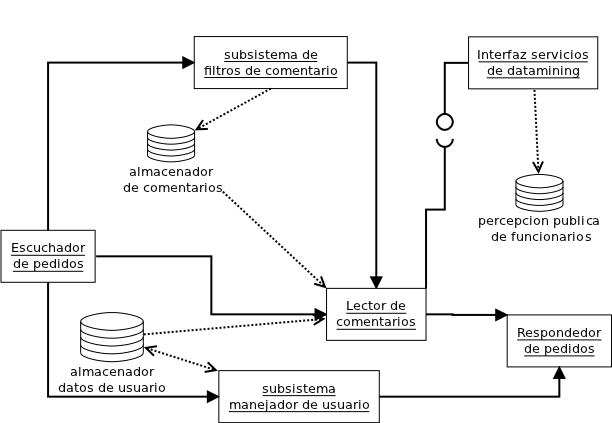
\includegraphics[scale=0.55]{../img/alto_nivel.png}\\
\end{center}

\begin{spacing}{1.5}
Como se muestra en la imagen el filtro escribirá en el almacenador de comentarios todos los comentarios etiquetados (más adelante explicaremos la metodología para lograr esto). La idea de la etiquetación es obtener una transformación de comentarios en cualquier formato a texto plano. Las ventajas de hacer esto y almacenarlo es que por un lado almacenamos todos los comentarios y son visibles para mostrarlos a la oposición si quisiera verificarlos. 
Además, al estar etiquetados si algún usuario configura que no le gustan algúna palabra en especial, se puede filtrar todos los comentarios que contengan una etiqueta con esa palabra. Para que el lector sepa de la configuración de cada usuario es necesario poder realizar lecturas al alamacenador de datos de usuarios.
\end{spacing}

\begin{center}
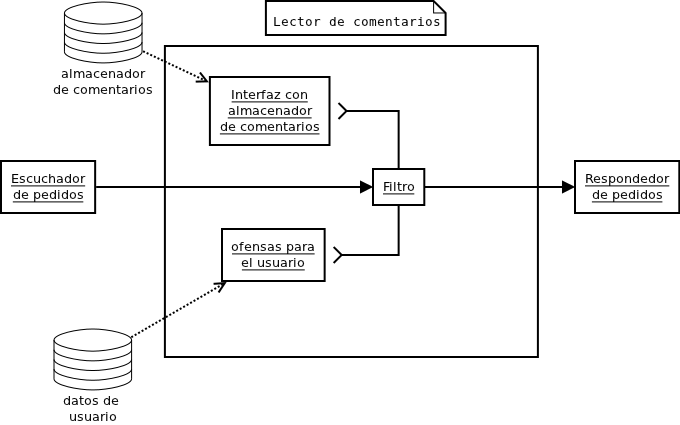
\includegraphics[scale=0.45]{../img/lectura.png}\\
\end{center}
\begin{center}
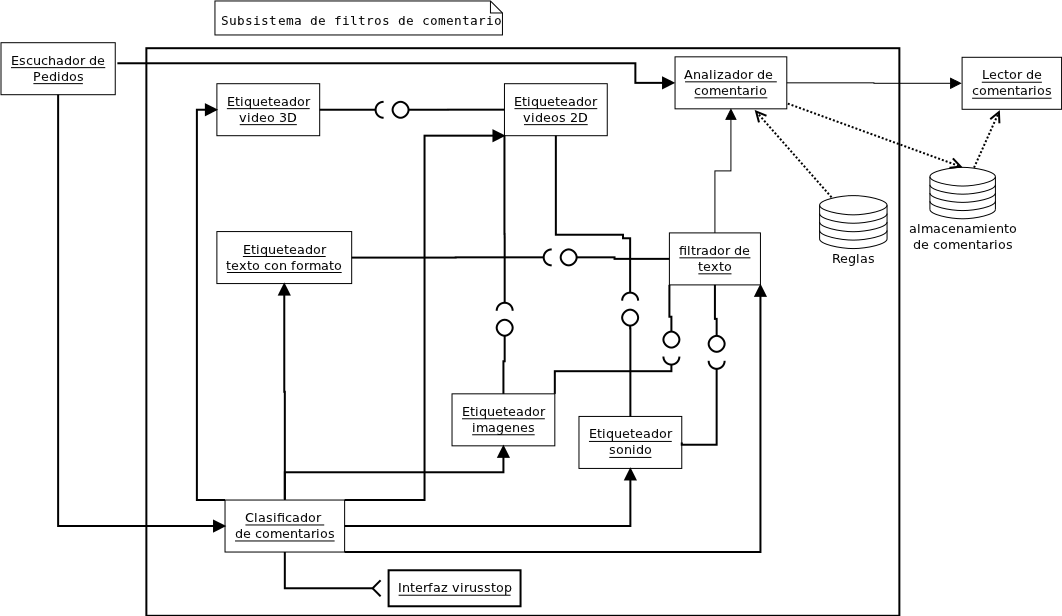
\includegraphics[scale=0.45]{../img/filtros.png}\\
\end{center}
\begin{center}
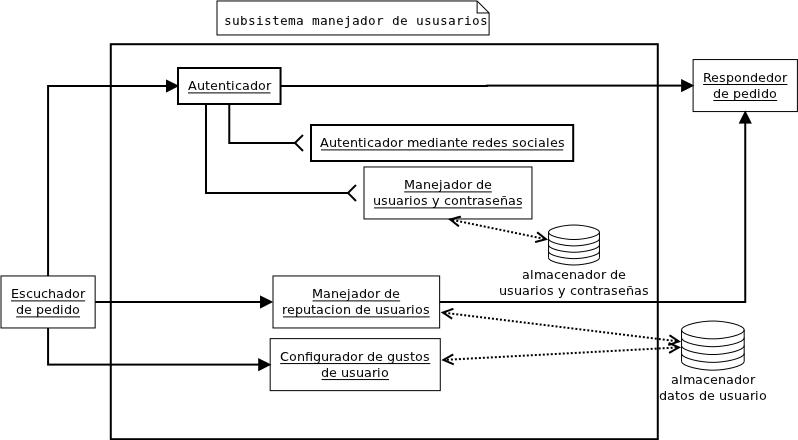
\includegraphics[scale=0.5]{../img/autenticador.png}\\
\end{center}

